\chapter{混合式双轮足机器人机械结构设计}\label{chap:mechanism}

双轮足机器人的控制效果很大程度上取决于机械本体。若腿部惯量过大、传动回差明显，后续的平衡控制和腿长调节都会变得困难。因此，本章先给出样机的设计指标，再说明腿部、躯干、传动、轮组、电机和传感器的具体选型，为第三章建模提供必要的结构参数。

\section{设计目标与需求分析}

样机主要面向平地移动、低台阶越障和原地平衡等场景。与四足轮腿平台相比，双轮足结构的执行器数量较少，整机也更紧凑；相应地，它对重心位置、腿部刚度和姿态反馈更敏感。结合后续控制实验的需要，机械设计需满足以下要求：

\begin{enumerate}
  \item 移动与越障能力：机器人在轮式支撑状态下应能达到目标速度，并通过腿部伸缩完成低台阶越障和落地缓冲。
  \item 轻量化：整机质量控制在较低水平，尤其要减小腿部运动件的转动惯量，避免电机长期工作在高负载区间。
  \item 刚度与装配精度：腿部机构、髋部轴系和传动系统需有足够刚度，传动间隙也应控制在可接受范围内。
  \item 集成与维护：躯干需要容纳电池、主控板、驱动器和传感器，并留出装配、走线和后续调试空间。
  \item 便于建模：机械构型应能用虚拟腿长和虚拟腿摆角描述，以便第三章建立任务空间模型。
\end{enumerate}

样机预期性能指标见\tabref{tab:design-targets}。其中，整机质量和自由度用于限制平台复杂度，移动速度和越障高度对应主要运动能力，连续工作时间用于约束电池和整机效率。

\begin{table}[H]
  \centering
  \caption{样机预期性能指标}\label{tab:design-targets}
  \renewcommand{\arraystretch}{1.3}
  \begin{tabular}{p{3cm}p{3cm}p{7cm}}
    \toprule
    指标名称 & 期望目标值 & 说明 \\
    \midrule
    整机质量 & $\leq 5\,\mathrm{kg}$ & 降低惯性和能耗，提高平衡控制响应速度 \\
    移动速度 & $\geq 2\,\mathrm{m/s}$ & 轮式移动能力要求 \\
    可跨越台阶高度 & $\geq 10\,\mathrm{cm}$ & 腿部伸缩能力要求 \\
    自由度 & $6\,\mathrm{DOF}$ & 左右腿部驱动与双轮驱动的基本配置 \\
    连续工作时间 & $\geq 30\,\mathrm{min}$ & 电池容量和整机效率约束 \\
    \bottomrule
  \end{tabular}
\end{table}

总体结构由躯干、左右对称腿部模块和两个驱动轮组成。腿部采用混合式闭环连杆机构，在串联主链中加入局部并联支链，以兼顾运动范围和支撑刚度。腿部驱动电机布置在靠近躯干的位置，通过链传动带动连杆运动；轮毂电机布置在足端，用于平地移动和差速转向。

\section{腿部结构设计}

腿部结构决定了越障高度、支撑刚度以及后续任务空间变量的定义。每条腿由髋部基座、主动曲柄、从动连杆、闭环支链和足端轮组构成。该结构保留了串联腿的运动范围，同时通过闭环支链提高局部刚度，适合小型双轮足样机。

\begin{figure}[H]
  \centering
  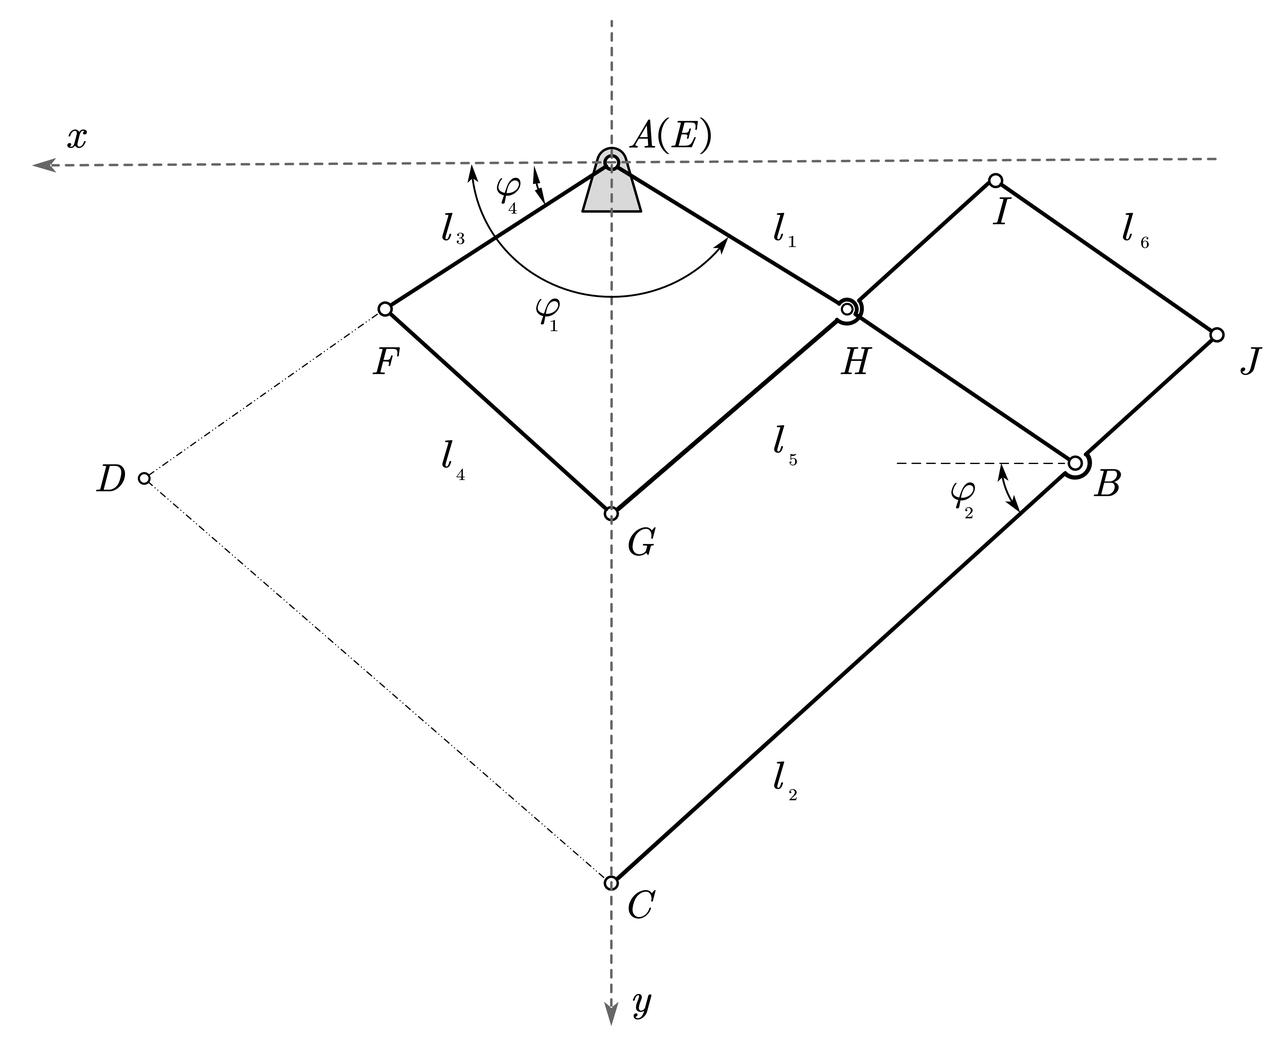
\includegraphics[width=0.52\textwidth]{figures/ch02/image1.png}
  \caption{腿部连杆机构简图}
  \label{fig:leg-linkage}
\end{figure}

为减小腿部转动惯量，腿部主要驱动电机布置在髋关节附近，并尽量靠近躯干。这样在摆腿、落地缓冲和越障时，质量较大的电机本体不随足端大幅运动，可降低惯性力矩和冲击载荷。足端轮组同时承担支撑和驱动作用，与连杆机构一起构成轮足复合运动单元。

根据整机尺寸和越障指标，腿部连杆尺寸需要同时满足伸展高度、收缩高度和传动角约束。选取的关键尺寸如下：

\begin{itemize}
  \item 驱动曲柄长度：$AF = AH = 86.4\,\mathrm{mm}$，该尺寸影响腿部摆动幅度和电机输出端力臂。
  \item 从动连杆长度：$CJ = 250.16\,\mathrm{mm}$，该尺寸用于保证足端伸展范围。
  \item 主支撑杆长度：$GI = 160\,\mathrm{mm}$，该尺寸用于形成主要承载支链。
\end{itemize}

当腿部机构接近最大伸展姿态时，可估算足端最大高度为

\begin{equation}
  H_{\max} = AB + BC = 160 + 196 = 356\,\mathrm{mm}.
\end{equation}

受机械限位和传动角限制，设定曲柄向上旋转的极限夹角约为水平以上 $30^\circ$，此时腿部最小收缩高度约为

\begin{equation}
  H_{\min} \approx 100\,\mathrm{mm}.
\end{equation}

由此得到腿部有效伸缩行程为

\begin{equation}
  S_{\mathrm{eff}} = H_{\max} - H_{\min} \approx 256\,\mathrm{mm}.
\end{equation}

该行程大于\tabref{tab:design-targets}中的越障高度指标，也为落地缓冲和高度调节留出余量。由上述参数得到的腿部工作空间如\figref{fig:leg-workspace}所示，足端在竖直方向上的可达范围满足后续虚拟腿建模需要。

\begin{figure}[H]
  \centering
  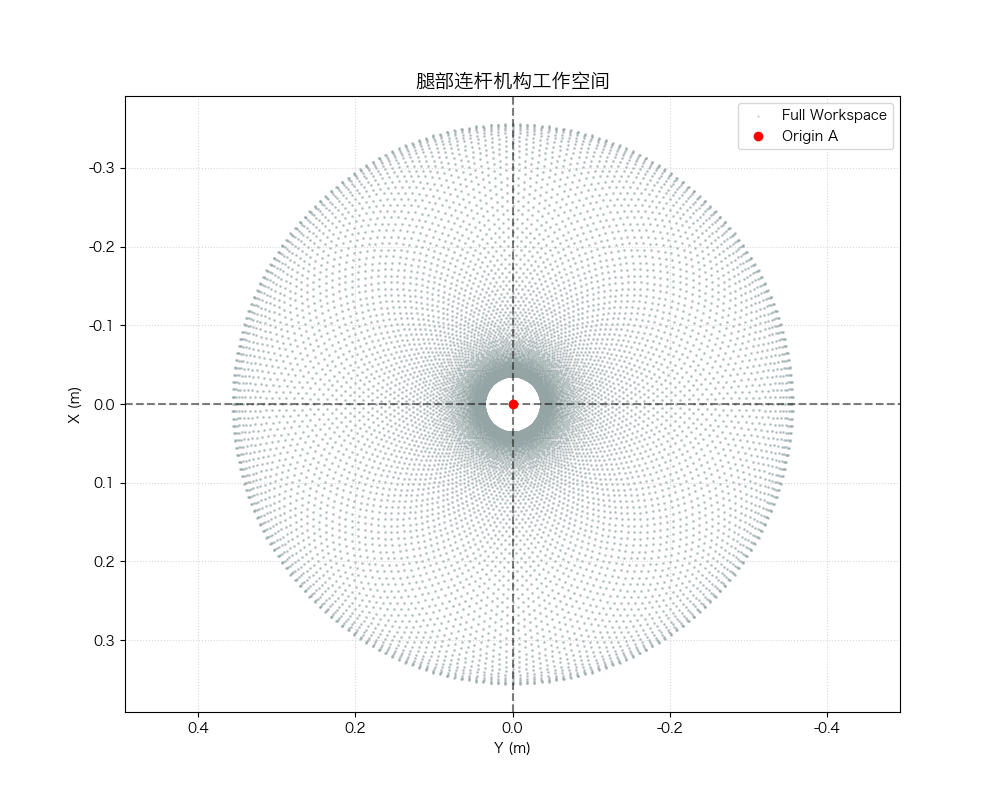
\includegraphics[width=0.72\textwidth]{figures/ch02/image2.png}
  \caption{腿部连杆工作空间示意图}
  \label{fig:leg-workspace}
\end{figure}

腿部连杆参数汇总如\tabref{tab:link-lengths}所示。第三章将根据这些几何参数建立闭环运动学模型。

\begin{table}[H]
  \centering
  \caption{腿部连杆参数汇总}\label{tab:link-lengths}
  \renewcommand{\arraystretch}{1.2}
  \begin{tabular}{cc}
    \toprule
    连杆代号 & 长度/m \\
    \midrule
    AF & 0.08640 \\
    FG & 0.10584 \\
    GI & 0.16000 \\
    IJ & 0.07360 \\
    JC & 0.25016 \\
    AB & 0.16000 \\
    \bottomrule
  \end{tabular}
\end{table}

\begin{figure}[H]
  \centering
  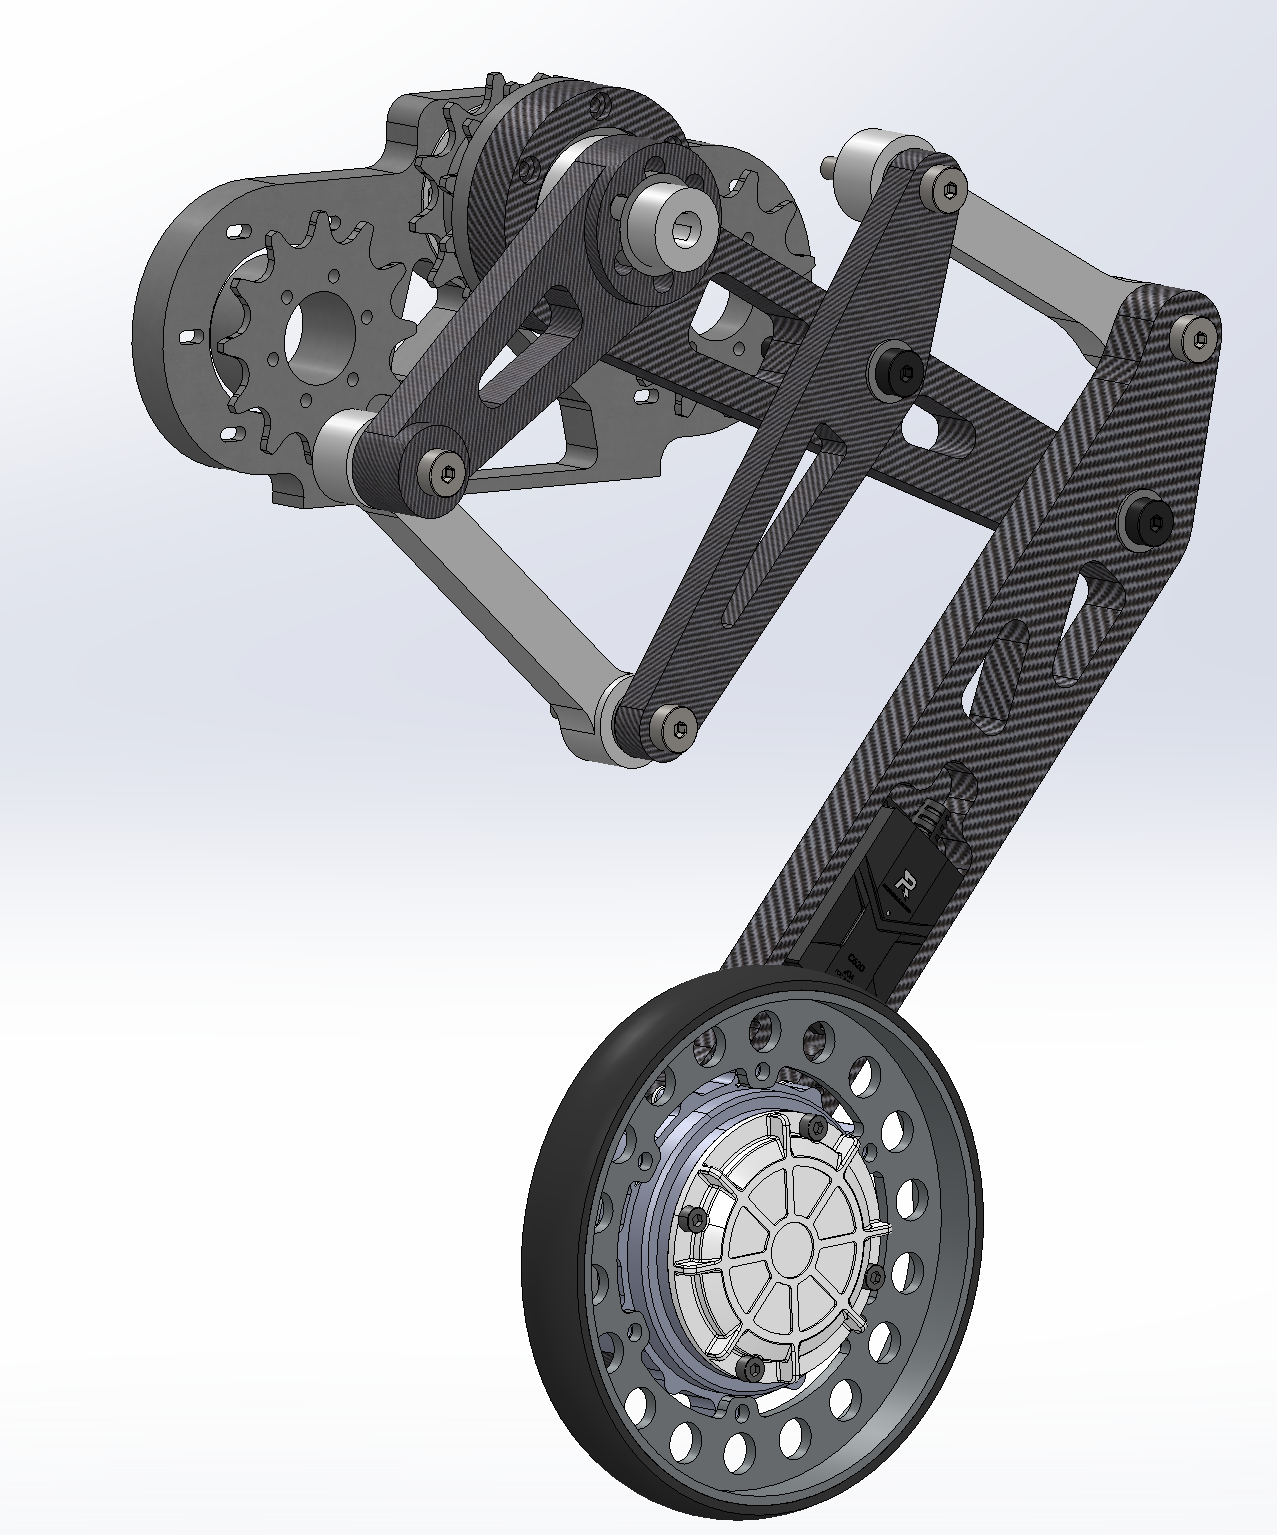
\includegraphics[width=0.6\textwidth]{figures/ch02/image3.png}
  \caption{腿部结构局部设计示意图}
  \label{fig:leg-detail}
\end{figure}

\section{躯干结构设计}

躯干承担主要承载、安装和供电功能，也是左右腿部模块的连接基座。由于双轮足机器人本身欠驱动，躯干质量分布会直接影响平衡控制难度。本文采用框架式躯干结构，在留出安装空间的同时控制质量和重心高度。

左右髋关节安装结构与躯干框架一体设计。两侧髋部之间采用镂空板材连接，形成近似箱式的承载结构；躯干上方安装 3D 打印电池架，便于固定和拆装电池；主控板、电源模块和驱动器布置在躯干内部或侧面安装区域。这样可以让腿部驱动电机、电池和控制硬件尽量靠近整机中心，减少不必要的偏置载荷。

\begin{figure}[H]
  \centering
  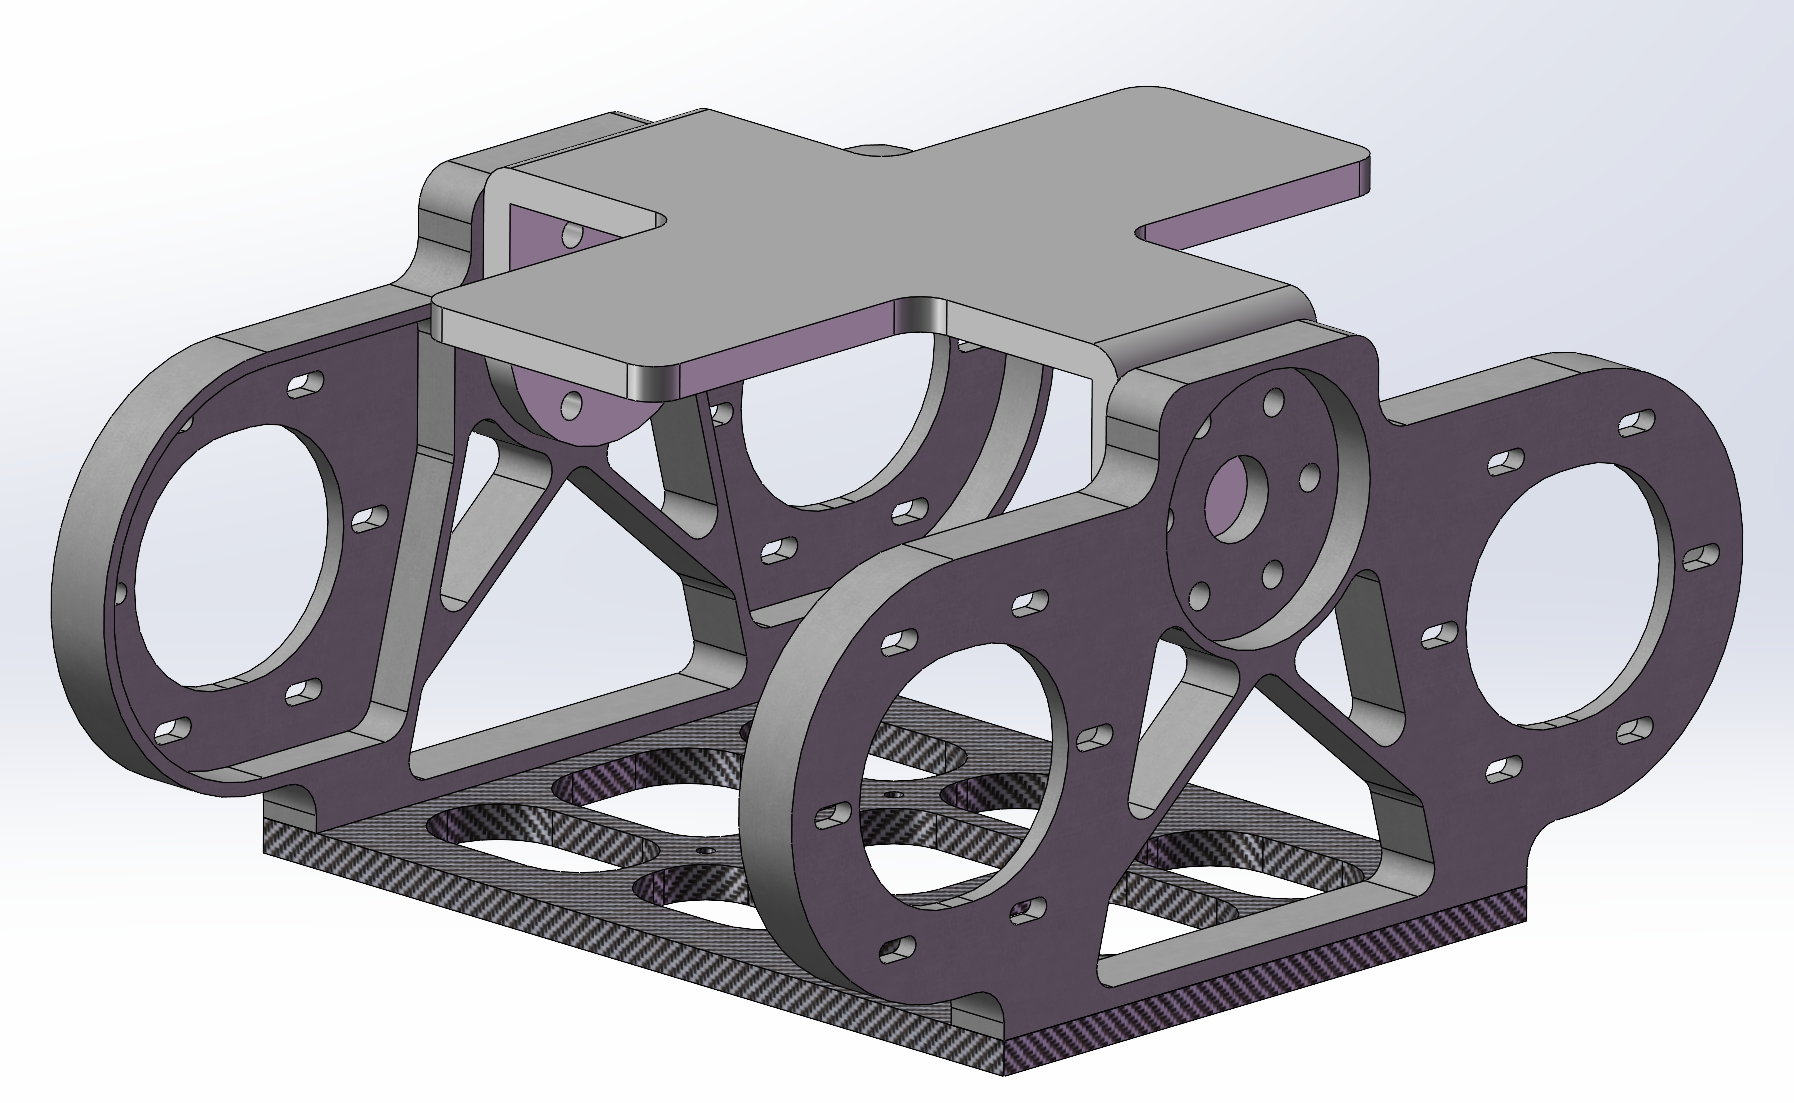
\includegraphics[width=0.6\textwidth]{figures/ch02/image4.png}
  \caption{躯干结构设计示意图}
  \label{fig:body-structure}
\end{figure}

主要承载板件优先采用碳纤维板材或 7075/6061 铝合金加工。碳纤维板材比刚度较高，适合用于侧板和连接板；铝合金更适合轴承座、电机座等需要较高加工精度的部位。电池架、线束固定件等非主要受力部件采用 3D 打印件，便于快速修改结构。

惯性测量单元尽量安装在靠近机体几何中心的位置，以减小局部振动和结构弹性对姿态测量的影响。电池和驱动器也尽量对称布置，避免左右腿支撑力出现明显静态偏差。

\section{传动系统设计}

传动系统负责把躯干附近电机的输出力矩传递到腿部连杆。设计时需控制传动回差和弹性变形，同时避免引入过多附加质量。本文传动部分包括髋关节嵌套轴系和链传动。

\subsection{髋关节轴系设计}

髋关节轴系采用嵌套式二级轴系，通过内外两层转动轴和两组轴承传递不同自由度的力矩。内轴系主要传递膝关节相关驱动力矩，外轴系支撑髋部连杆运动。该结构横向尺寸较小，适合布置在双腿之间的有限空间内。

\begin{figure}[H]
  \centering
  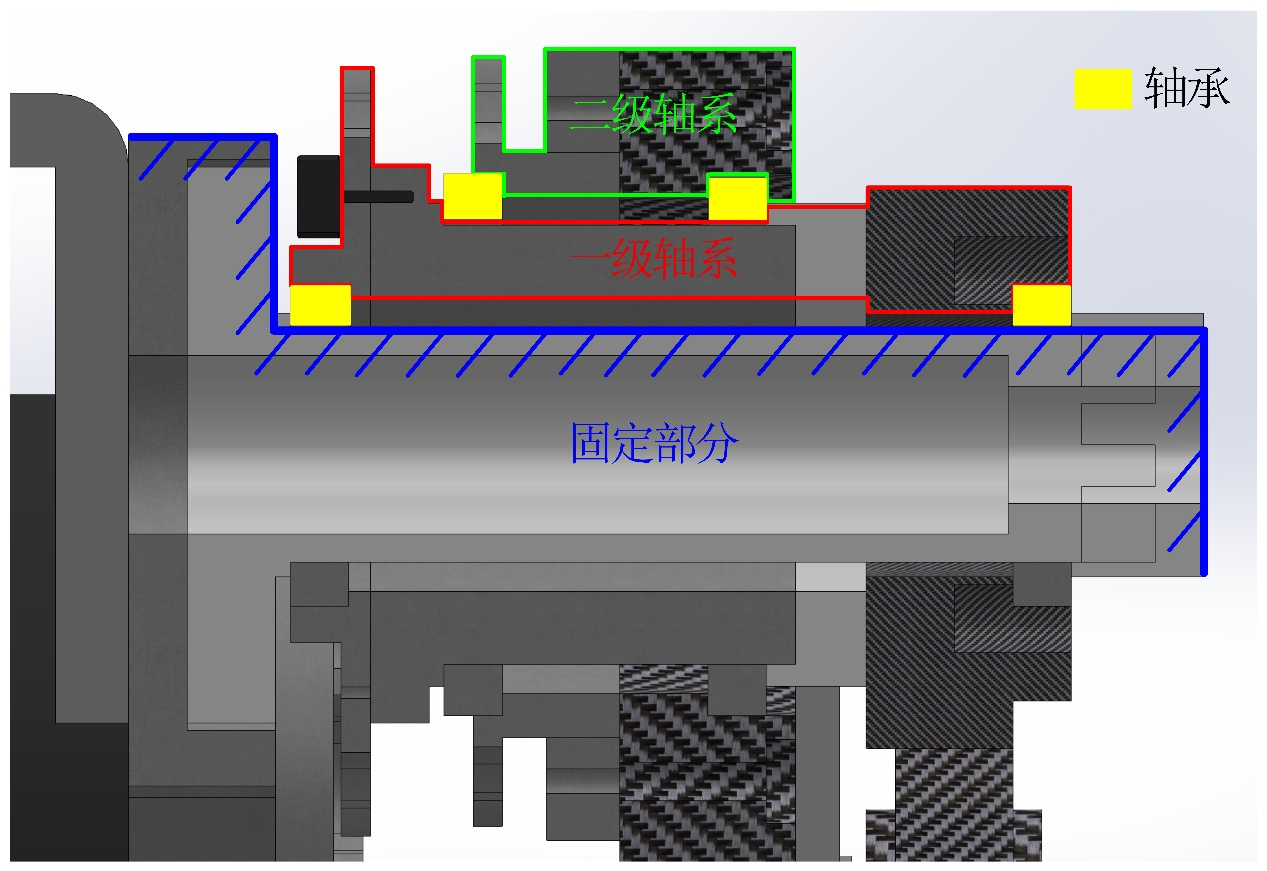
\includegraphics[width=0.8\textwidth]{figures/ch02/image5.jpeg}
  \caption{髋关节嵌套轴系结构示意图}
  \label{fig:hip-axis}
\end{figure}

与将电机直接安装在腿部远端相比，嵌套轴系配合后置电机可减小腿部摆动部件质量。该方案对装配精度和轴系同轴度要求更高，因此加工时需要保证轴承座定位精度，并通过预紧减小轴向间隙。

\subsection{链传动设计与校核}

腿部力矩传递采用 9 速自行车链条。与同步带相比，滚子链属于啮合传动，平均传动比更稳定，抗拉强度也更高；与常见工业链条相比，自行车链条宽度较小，有利于控制腿部横向尺寸。

在跳跃落地或快速伸腿工况下，链条会承受较大的瞬时拉力。以腿部电机说明书给出的峰值扭矩 $T_{\text{peak}} = 7\,\mathrm{N\cdot m}$、链轮等效直径 $d = 0.04907\,\mathrm{m}$ 估算，有效圆周力为

\begin{equation}
  F_t = \frac{2 T_{\text{peak}}}{d}
  = \frac{2 \times 7}{0.04907}
  \approx 285.3\,\mathrm{N}.
\end{equation}

主流 9 速自行车链条的最小破坏载荷通常可达到

\begin{equation}
  F_u \geq 8500\,\mathrm{N}.
\end{equation}

由此可得静强度安全系数

\begin{equation}
  S = \frac{F_u}{F_t}
  = \frac{8500}{285.3}
  \approx 29.79.
\end{equation}

即使考虑冲击载荷系数 $K_A \approx 1.5$，链条强度仍有余量。

\begin{figure}[H]
  \centering
  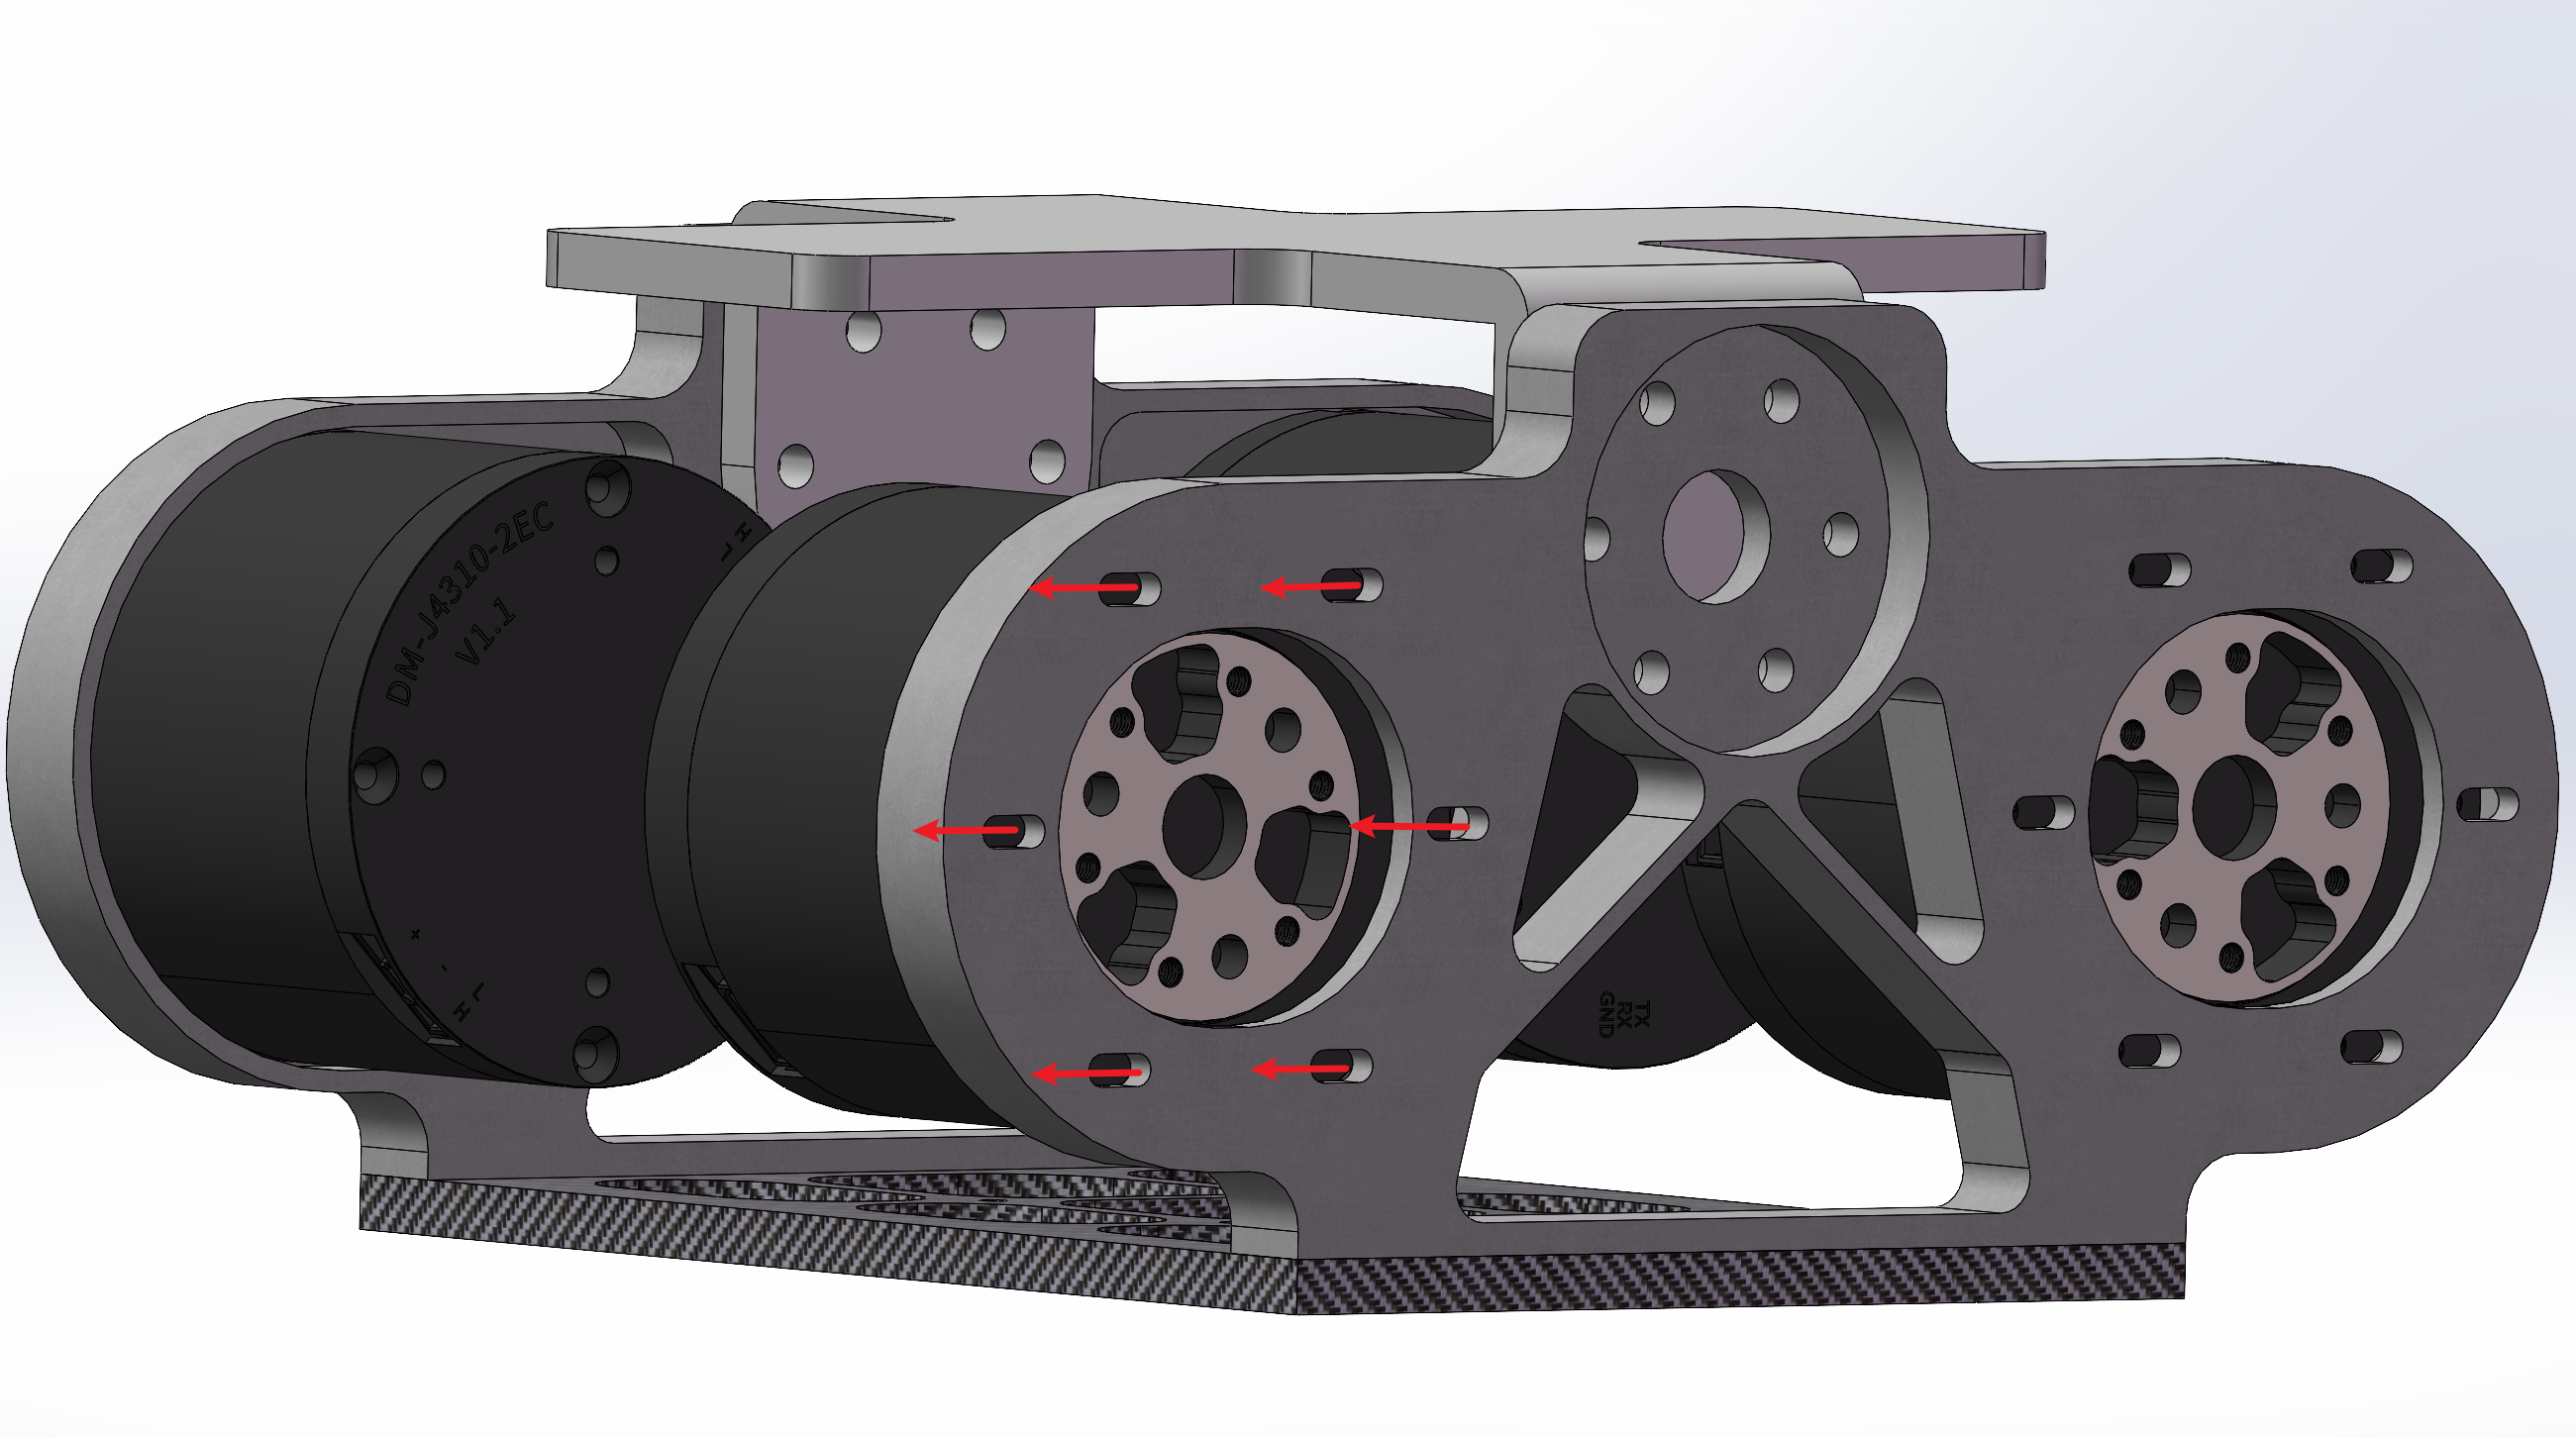
\includegraphics[width=0.8\textwidth]{figures/ch02/image6.png}
  \caption{髋关节连接板滑槽示意图}
  \label{fig:chain-drive}
\end{figure}

链条长期工作后会因销轴和套筒磨损而变长。链条过松会增大传动回差，影响倒立摆平衡控制，也会在冲击工况下增加脱链风险。为避免增加弹簧张紧臂或惰轮机构，本文通过改变中心距完成张紧：在髋关节连接板上将电机安装孔设计为水平滑槽，滑槽长度为 $7\,\mathrm{mm}$，允许电机定子沿水平方向进行约 $\pm 4\,\mathrm{mm}$ 的位置调整。这样不需要增加额外运动部件，维护时也比较直接。

\section{轮组系统设计}

轮组用于平地移动和差速转向。驱动轮直接集成在腿部末端，既是轮式模式下的支撑点，也是虚拟腿末端点。该布置省去了额外足端传动机构，可降低结构复杂度和质量。

\begin{figure}[H]
  \centering
  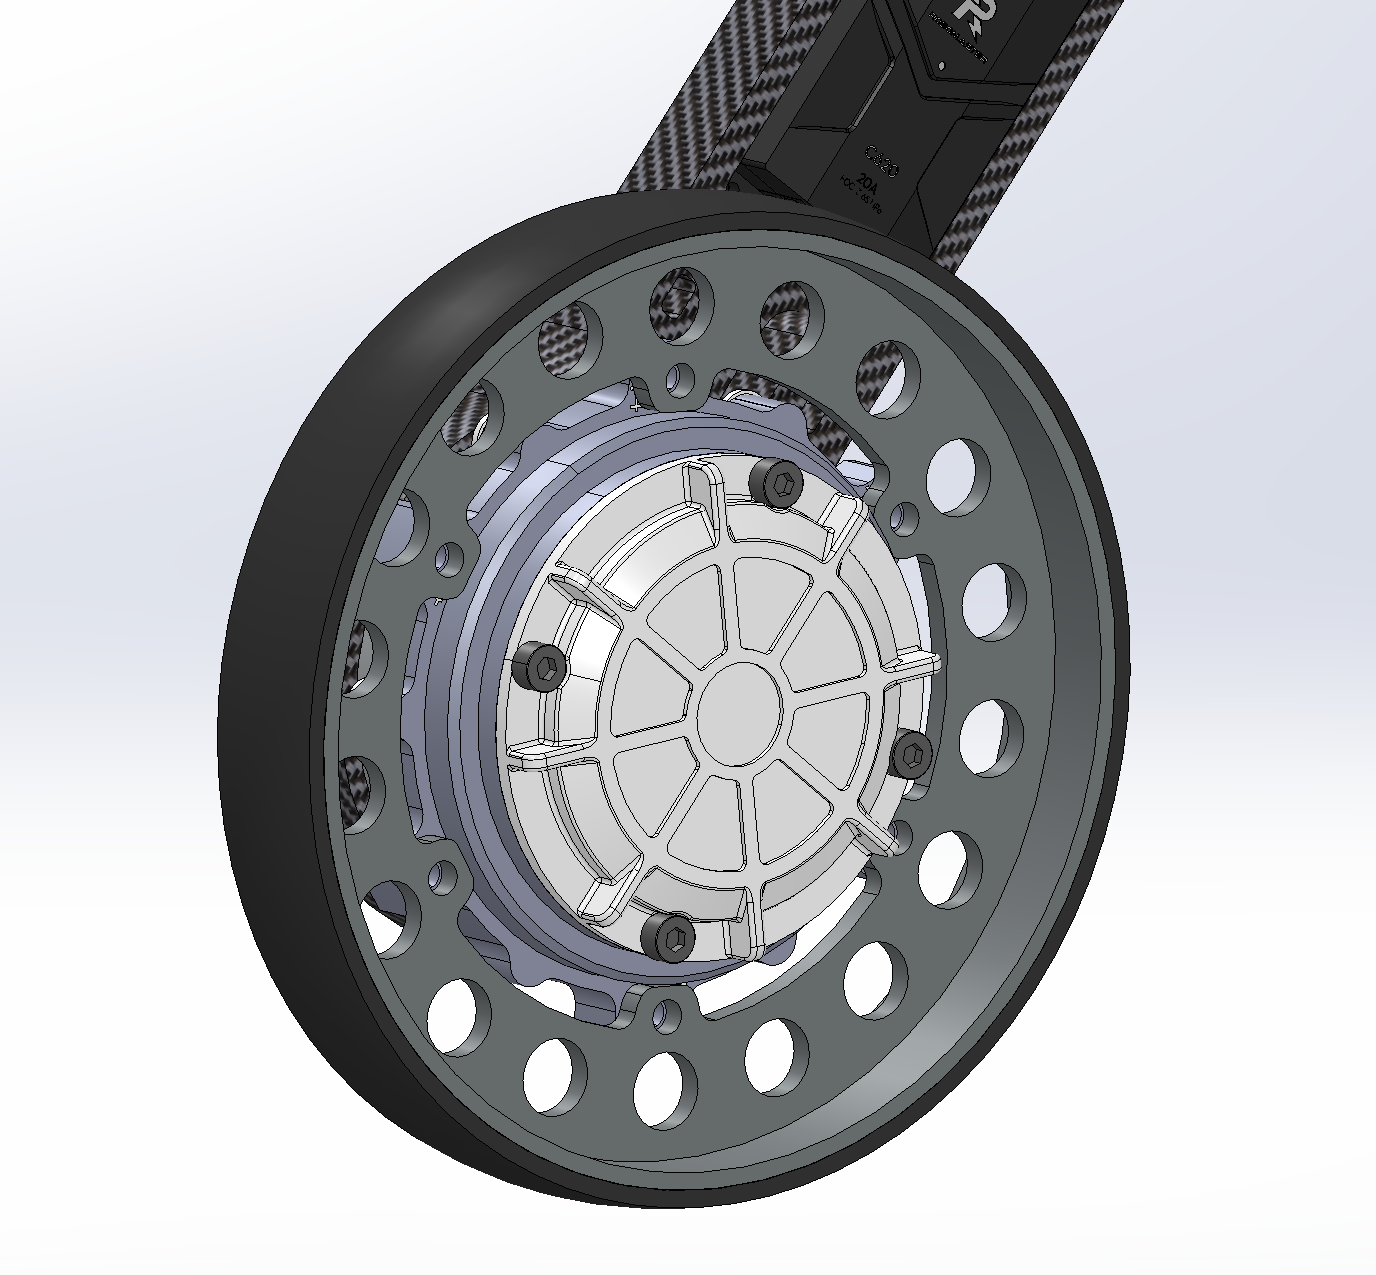
\includegraphics[width=0.5\textwidth]{figures/ch02/image9.png}
  \caption{足端轮组结构示意图}
  \label{fig:wheel-module}
\end{figure}

设轮子半径为 $r = 0.06\,\mathrm{m}$，根据最大移动速度指标 $v_{\max} \geq 2\,\mathrm{m/s}$，轮组所需角速度为

\begin{equation}
  \omega = \frac{v_{\max}}{r}
  = \frac{2}{0.06}
  \approx 33.3\,\mathrm{rad/s}
  \approx 318\,\mathrm{RPM}.
\end{equation}

若机器人在 $0.5\,\mathrm{s}$ 内由静止加速至 $2\,\mathrm{m/s}$，所需加速度为

\begin{equation}
  a = 4\,\mathrm{m/s^2}.
\end{equation}

当整机质量取 $M = 5\,\mathrm{kg}$、滚动阻力系数取 $\mu = 0.05$ 时，总牵引力需求为

\begin{equation}
  F_{\text{total}} = Ma + \mu Mg
  = 20 + 0.05 \times 5 \times 9.8
  = 22.45\,\mathrm{N}.
\end{equation}

对应轮组总扭矩为

\begin{equation}
  T_{\text{acc}} = F_{\text{total}} r
  = 22.45 \times 0.06
  \approx 1.35\,\mathrm{N\cdot m}.
\end{equation}

在爬坡工况下，若坡度取 $\alpha = 20^\circ$，重力沿坡面方向的分量为

\begin{equation}
  F_{\text{climb}} = Mg \sin \alpha
  = 5 \times 9.8 \times 0.342
  \approx 16.8\,\mathrm{N},
\end{equation}

对应爬坡扭矩为

\begin{equation}
  T_{\text{climb}} = F_{\text{climb}} r
  = 16.8 \times 0.06
  \approx 1.01\,\mathrm{N\cdot m}.
\end{equation}

双轮驱动时，单轮连续扭矩需求约为 $0.7 \sim 1.0\,\mathrm{N\cdot m}$。考虑加速、坡面扰动和控制裕度后，选用额定扭矩为 $2.5\,\mathrm{N\cdot m}$ 的减速轮毂电机。

\section{电机选型与校核}

执行器包括腿部关节电机和足端轮毂电机。腿部电机承担站立支撑、腿部伸缩和越障任务，轮毂电机承担轮式移动和差速转向任务。由于控制系统需要实时运行，电机需支持力矩控制，并具备足够的峰值扭矩。

\subsection{腿部关节电机}

腿部关节电机按跳跃起跳、落地缓冲和单腿支撑等工况估算。下文用跳跃起跳估算峰值扭矩，用半蹲支撑估算额定扭矩。

假设机器人需要实现原地跳跃，目标腾空高度为 $H_{\text{jump}} = 0.3\,\mathrm{m}$。根据能量守恒，机器人离地瞬间速度满足

\begin{equation}
  \frac{1}{2} M v_{\text{takeoff}}^2 = M g H_{\text{jump}},
\end{equation}

解得

\begin{equation}
  v_{\text{takeoff}} = \sqrt{2 g H_{\text{jump}}}
  \approx 2.42\,\mathrm{m/s}.
\end{equation}

若起跳阶段有效伸腿行程取 $h_{\text{acc}} = 0.15\,\mathrm{m}$，由动能定理可得地面对足端的平均反作用力

\begin{equation}
  F_{\text{ground}} =
  \frac{M g H_{\text{jump}}}{h_{\text{acc}}} + Mg
  = \frac{5 \times 9.8 \times 0.3}{0.15} + 49
  = 147\,\mathrm{N}.
\end{equation}

根据虚功原理，足端力与关节力矩满足 $\boldsymbol{\tau} = \boldsymbol{J}^{\mathsf{T}}\boldsymbol{F}$。在典型半蹲姿态下，设等效连杆长度为 $L_{\text{link}} \approx 0.15\,\mathrm{m}$，有效力臂系数取 0.7，则峰值关节力矩可估算为

\begin{equation}
  T_{\text{peak}} \approx
  F_{\text{ground}} L_{\text{link}} \times 0.7
  \approx 147 \times 0.15 \times 0.7
  \approx 15.4\,\mathrm{N\cdot m}.
\end{equation}

上述估算按较保守的工况取值。实际样机为双腿协同支撑，且每条腿由两个主动关节电机和闭环连杆机构共同承担负载，单电机峰值需求会低于该估算。综合质量、体积和控制接口，腿部关节驱动器选用额定扭矩 $3\,\mathrm{N\cdot m}$、峰值扭矩 $7\,\mathrm{N\cdot m}$ 的无刷减速电机。该电机支持 MIT、速度和位置控制模式，满足站立平衡和腿部快速调节需求。

\begin{figure}[H]
  \centering
  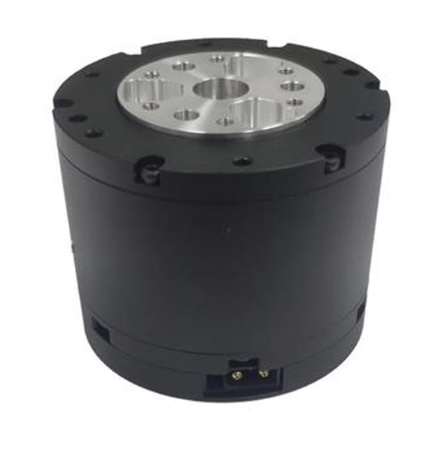
\includegraphics[width=0.4\textwidth]{figures/ch02/image7.jpg}
  \caption{腿部关节驱动电机}
  \label{fig:leg-motor}
\end{figure}

\begin{table}[H]
  \centering
  \caption{腿部关节驱动电机关键参数}
  \label{tab:leg-motor-parameters}
  \begin{tabular}{lcc}
    \toprule
    参数 & 数值 & 说明 \\
    \midrule
    额定扭矩 & $3\,\mathrm{N\cdot m}$ & 连续输出扭矩 \\
    峰值扭矩 & $7\,\mathrm{N\cdot m}$ & 短时输出扭矩 \\
    额定转速 & $120\,\mathrm{r/min}$ & 减速后输出转速 \\
    空载最大转速 & $200\,\mathrm{r/min}$ & 空载工况 \\
    减速比 & $10:1$ & 内置减速机构 \\
    电机质量 & 约 $300\,\mathrm{g}$ & 单个电机 \\
    \bottomrule
  \end{tabular}
\end{table}

对于静态或准静态半蹲支撑工况，若按单腿支撑整机重量进行保守估算，有

\begin{equation}
  T_{\text{rated}} =
  Mg L_{\text{link}} \sin 45^\circ
  \approx 5 \times 9.8 \times 0.15 \times 0.707
  \approx 5.2\,\mathrm{N\cdot m}.
\end{equation}

双腿支撑时，单腿持续负载约减半，即约为 $2.6\,\mathrm{N\cdot m}$。所选电机额定扭矩为 $3\,\mathrm{N\cdot m}$，可覆盖该需求，并为姿态调节和小扰动恢复留出余量。

\subsection{轮毂电机}

轮毂电机按第 2.5 节的速度、加速和爬坡需求选型。本文选用额定扭矩为 $2.46\,\mathrm{N\cdot m}$ 的 M3508 减速轮毂电机，并将其直接布置在足端轮组内部。该方案省去额外传动链，轮系角度和速度也可直接用于估计前进位移与速度。

\begin{figure}[H]
  \centering
  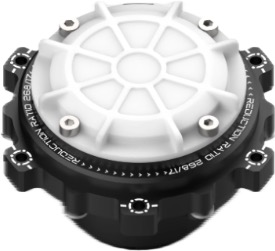
\includegraphics[width=0.3\textwidth]{figures/ch02/image8_safe.jpg}
  \caption{足端轮毂电机}
  \label{fig:wheel-motor}
\end{figure}

\begin{table}[H]
  \centering
  \caption{足端轮毂电机关键参数}
  \label{tab:wheel-motor-parameters}
  \begin{tabular}{lcc}
    \toprule
    参数 & 数值 & 说明 \\
    \midrule
    额定扭矩 & $2.46\,\mathrm{N\cdot m}$ & 减速箱输出端 \\
    堵转扭矩 & $3.69\,\mathrm{N\cdot m}$ & 短时极限输出 \\
    额定转速 & $571\,\mathrm{r/min}$ & 减速后输出转速 \\
    空载转速 & $587\,\mathrm{r/min}$ & 空载工况 \\
    最大效率 & $70\%$ & 电机效率 \\
    电机质量 & $336.4\,\mathrm{g}$ & 单个电机 \\
    \bottomrule
  \end{tabular}
\end{table}

根据前述计算，双轮驱动下单轮连续扭矩需求约为 $0.7 \sim 1.0\,\mathrm{N\cdot m}$，所选轮毂电机额定扭矩为 $2.46\,\mathrm{N\cdot m}$，可满足平地加速和一定坡度爬升需求。直接驱动形式还能减少传动回差，使轮系状态估计更简单。

\section{本章小结}

本章完成了样机机械结构设计。根据平衡移动、越障、轻量化和嵌入式实时控制需求，确定了整机质量、自由度、移动速度和越障高度等指标；设计了带闭环支链的混合式腿部机构，并通过连杆尺寸和工作空间分析验证其伸缩范围；给出了躯干、髋关节轴系、链传动和足端轮组方案，并对链条强度、腿部关节电机和轮毂电机进行了估算校核。

最终样机采用躯干集中承载、混合式腿部支撑调节、足端轮组驱动移动的结构。第三章将基于该结构建立运动学和动力学模型。
